\documentclass[tikz,border=4pt]{standalone}
% Shared style for every figure and for the deck: one accent, one
% highlight, thin lines, rounded nodes, nothing decorative.
\usepackage[T1]{fontenc}
\usepackage{lmodern}
\renewcommand{\familydefault}{\sfdefault}
\usepackage{tikz}
\usetikzlibrary{arrows.meta,positioning,calc,shapes.misc,fit,backgrounds,decorations.pathreplacing}
\definecolor{ink}{RGB}{40,40,40}
\definecolor{soft}{RGB}{150,150,150}
\definecolor{faint}{RGB}{225,225,225}
\definecolor{accent}{RGB}{0,95,115}
\definecolor{accentlight}{RGB}{214,232,236}
\definecolor{warn}{RGB}{196,84,40}
\definecolor{warnlight}{RGB}{247,226,216}
\tikzset{
  every picture/.style={color=ink, line width=0.5pt, font=\small},
  node distance=12mm and 18mm,
  box/.style={draw=ink, rounded corners=2pt, fill=white, inner sep=5pt, minimum height=7mm, align=center},
  maker/.style={box, minimum width=18mm},
  cat/.style={box, inner sep=3.5pt, minimum height=6mm},
  root/.style={box, fill=accentlight, draw=accent},
  bad/.style={box, fill=warnlight, draw=warn},
  ghost/.style={box, draw=soft, text=soft, dashed},
  flow/.style={-{Stealth[length=4pt,width=3.5pt]}, line width=0.5pt},
  sub/.style={-{Stealth[length=4pt,width=3.5pt]}, line width=0.5pt, color=soft},
  strong/.style={flow, color=accent, line width=0.8pt},
  wrong/.style={flow, color=warn},
  lbl/.style={font=\footnotesize, text=ink, inner sep=1.5pt, fill=white},
  note/.style={font=\footnotesize, text=soft, align=center},
  rate/.style={font=\footnotesize, text=accent, inner sep=1pt, fill=white},
}

\usepackage{amsmath}
\usepackage{pgfplots}
\pgfplotsset{compat=1.17}

\begin{document}
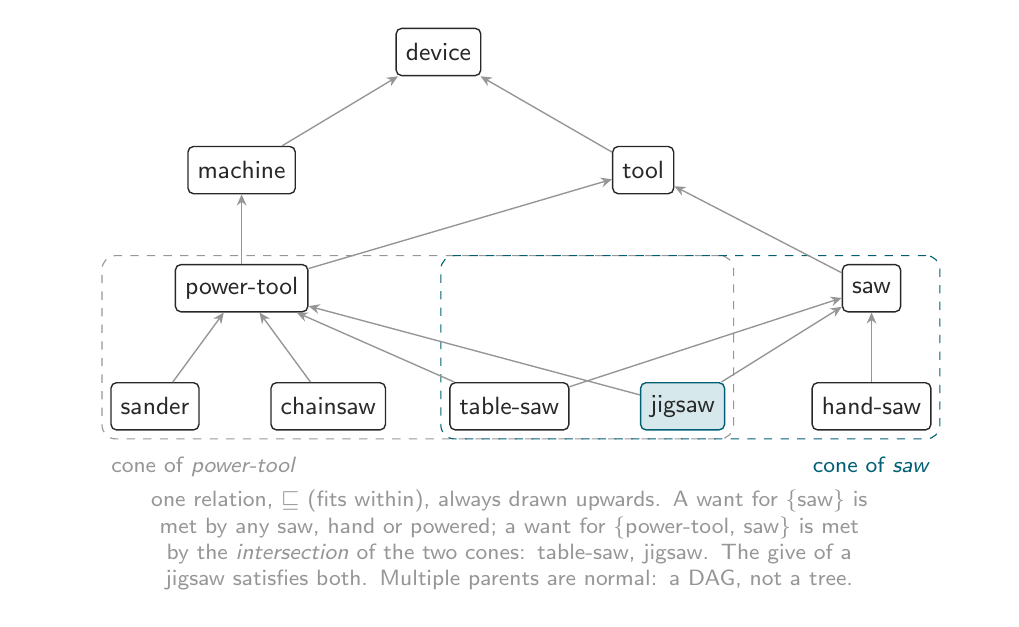
\begin{tikzpicture}
  % One order, drawn one way: supercategories above, subcategories below.
  % A want is a conjunction of categories; it is met by anything in the
  % intersection of their cones. Coordinates are explicit so that neither
  % cone's box swallows the other cone's apex.
  \node[cat] (sander)   at (0mm,0)  {sander};
  \node[cat] (chainsaw) at (22mm,0) {chainsaw};
  \node[cat] (table)    at (45mm,0) {table-saw};
  \node[cat, fill=accentlight, draw=accent] (jigsaw) at (67mm,0) {jigsaw};
  \node[cat] (hand)     at (91mm,0) {hand-saw};
  \node[cat] (power) at (11mm,15mm) {power-tool};
  \node[cat] (saw)   at (91mm,15mm) {saw};
  \node[cat] (machine) at (11mm,30mm) {machine};
  \node[cat] (tool)    at (62mm,30mm) {tool};
  \node[cat] (device)  at (36mm,45mm) {device};
  \draw[sub] (machine) -- (device); \draw[sub] (tool) -- (device);
  \draw[sub] (power) -- (machine); \draw[sub] (power) -- (tool);
  \draw[sub] (saw) -- (tool);
  \draw[sub] (sander) -- (power); \draw[sub] (chainsaw) -- (power);
  \draw[sub] (table) -- (power); \draw[sub] (jigsaw) -- (power);
  \draw[sub] (table) -- (saw); \draw[sub] (jigsaw) -- (saw); \draw[sub] (hand) -- (saw);
  \begin{scope}[on background layer]
    \node[fit=(power)(sander)(chainsaw)(table)(jigsaw), rounded corners=5pt, draw=soft, dashed, inner sep=3pt] (conepower) {};
    \node[fit=(saw)(table)(jigsaw)(hand), rounded corners=5pt, draw=accent, dashed, inner sep=3pt] (conesaw) {};
  \end{scope}
  \node[note, anchor=north west] at ($(conepower.south west) + (0,-1mm)$) {cone of \emph{power-tool}};
  \node[note, text=accent, anchor=north east] at ($(conesaw.south east) + (0,-1mm)$) {cone of \emph{saw}};
  \node[note, text width=120mm] at (45mm,-17mm) {one relation, $\sqsubseteq$ (fits within), always drawn upwards. A want for \{saw\} is met by any saw, hand or powered; a want for \{power-tool, saw\} is met by the \emph{intersection} of the two cones: table-saw, jigsaw. The give of a jigsaw satisfies both. Multiple parents are normal: a DAG, not a tree.};
\end{tikzpicture}
\end{document}
